\documentclass[conference]{IEEEtran}
\usepackage[T1]{fontenc}
\usepackage{graphicx}
\usepackage{booktabs}
\usepackage{siunitx}
\usepackage{amsmath,amssymb}
\usepackage{microtype}
\usepackage{xcolor}
\usepackage[hidelinks]{hyperref}
\usepackage[capitalise,noabbrev]{cleveref}
\usepackage{balance}
\sisetup{detect-all}
\graphicspath{{../figures/}}
\renewcommand{\topfraction}{0.9}
\renewcommand{\dbltopfraction}{0.9}
\renewcommand{\textfraction}{0.07}
\renewcommand{\floatpagefraction}{0.8}
\renewcommand{\dblfloatpagefraction}{0.8}
\setcounter{topnumber}{3}
\setcounter{dbltopnumber}{2}
% generated by scripts/make_numbers.py -- do not edit
\newcommand{\AWQcross}{175}
\newcommand{\AWQmaxEtoE}{2.44$\times$}
\newcommand{\AWQspeedup}{2.44$\times$}
\newcommand{\AccAWQFourteen}{93.9}
\newcommand{\AccAWQSeven}{90.4}
\newcommand{\AccBFFourteen}{n/a}
\newcommand{\AccBFSeven}{90.8}
\newcommand{\AccBFThree}{85.8}
\newcommand{\AccFPFourteen}{94.4}
\newcommand{\AccGPTQFourFourteen}{93.7}
\newcommand{\AccGPTQFourFourteenPct}{93.7}
\newcommand{\ActIntRatio}{1.6$\times$}
\newcommand{\BFmeas}{218}
\newcommand{\BWmeas}{1.61}
\newcommand{\BWutilVllm}{99}
\newcommand{\BackendFlipsSeven}{19}
\newcommand{\BackendFlipsThree}{38}
\newcommand{\BackendNoiseSeven}{0.4}
\newcommand{\BackendNoiseThree}{0.2}
\newcommand{\BonfAlpha}{0.0042}
\newcommand{\BusyBFone}{97}
\newcommand{\BusyIntone}{28}
\newcommand{\BusyNFone}{49}
\newcommand{\CVmax}{0.7}
\newcommand{\CVmed}{0.1}
\newcommand{\ClockAvg}{2812}
\newcommand{\DEightAbsSeven}{0.9}
\newcommand{\DEightAbsThree}{0.6}
\newcommand{\DFourMaxSeven}{$+0.2$}
\newcommand{\DFourMaxThree}{$-3.1$}
\newcommand{\DFourMinSeven}{$-0.5$}
\newcommand{\DFourMinThree}{$-3.8$}
\newcommand{\DeltaEightMax}{0.9}
\newcommand{\DeltaFourMax}{$+0.2$}
\newcommand{\DeltaFourMin}{$-0.5$}
\newcommand{\EightSentence}{the only nominally significant difference is an improvement (GPTQ-INT8 on 7B, $+0.9$ points, $p=0.043$), which does not survive a Bonferroni correction over the 12 comparisons}
\newcommand{\EmbedShareSeven}{14}
\newcommand{\EnAWQone}{1.9}
\newcommand{\EnBFmax}{0.21}
\newcommand{\EnBFone}{4.9}
\newcommand{\EnFPmax}{0.12}
\newcommand{\EnRatioAWQone}{2.5$\times$}
\newcommand{\ExcludedWindows}{2 windows, 26 minutes in total}
\newcommand{\FPeightmeas}{645}
\newcommand{\FPeightspeedup}{1.59$\times$}
\newcommand{\FPkernMmax}{1.9$\times$}
\newcommand{\FPkernMone}{1.8$\times$}
\newcommand{\FPmaxEtoE}{1.80$\times$}
\newcommand{\FPminEtoE}{1.59$\times$}
\newcommand{\FloorThree}{3.8}
\newcommand{\FourThreeSurvive}{3 of 3}
\newcommand{\FourteenNote}{In BF16 the 14B model's 29.5\,GB of weights leave no room for any KV cache even when vLLM may use 95\% of the GPU, so it cannot be served at all, while its AWQ-INT4 version runs with 82K cached tokens.}
\newcommand{\GPTQeightspeedup}{1.64$\times$}
\newcommand{\GuideHead}{Prefer a larger quantized model to a smaller full-precision one.}
\newcommand{\INTeightslowdown}{3.4$\times$}
\newcommand{\INTkernRange}{0.40--1.33$\times$}
\newcommand{\INTmaxEtoE}{0.71$\times$}
\newcommand{\INTminEtoE}{0.27$\times$}
\newcommand{\IntThreeOverSeven}{1.52$\times$}
\newcommand{\IntThreeWorst}{0.13$\times$}
\newcommand{\KVawqSeven}{355K}
\newcommand{\KVbfSeven}{187K}
\newcommand{\KVratioAWQ}{1.90$\times$}
\newcommand{\KernIntRatio}{3.7$\times$}
\newcommand{\LoadIntEightSeven}{12.5}
\newcommand{\LoadIntRatio}{7$\times$}
\newcommand{\MarlinEightCross}{164}
\newcommand{\MarlinEightMone}{1.9$\times$}
\newcommand{\MarlinFourCross}{333}
\newcommand{\MarlinFourMone}{3.2$\times$}
\newcommand{\MemBigInt}{1.04$\times$}
\newcommand{\MemBigNF}{1.49$\times$}
\newcommand{\MemSmallNF}{2.53$\times$}
\newcommand{\MinPEightSeven}{0.04}
\newcommand{\MinPEightThree}{0.32}
\newcommand{\ModelErrMax}{0.6}
\newcommand{\NFcross}{7}
\newcommand{\NFkernMmax}{0.58$\times$}
\newcommand{\NFkernMone}{2.39$\times$}
\newcommand{\NFsevenB}{1.13$\times$}
\newcommand{\NFslowdown}{1.39$\times$}
\newcommand{\NFthreeslow}{1.39$\times$}
\newcommand{\NaiveExcessMax}{54}
\newcommand{\NumMeasurements}{1{,}683}
\newcommand{\NumSig}{1 of 6}
\newcommand{\NumSigEightSeven}{1 of 3}
\newcommand{\NumSigEightThree}{0 of 3}
\newcommand{\NumSigFourSeven}{0 of 3}
\newcommand{\NumSigFourThree}{3 of 3}
\newcommand{\NumTests}{12}
\newcommand{\OutAWQOneLong}{2.42$\times$}
\newcommand{\OutAWQOneShort}{2.08$\times$}
\newcommand{\OutAWQSixteenLong}{2.16$\times$}
\newcommand{\OutAWQSixteenShort}{1.26$\times$}
\newcommand{\OutFPOneLong}{1.59$\times$}
\newcommand{\OutFPOneShort}{1.59$\times$}
\newcommand{\OutFPSixteenLong}{1.72$\times$}
\newcommand{\OutFPSixteenShort}{1.82$\times$}
\newcommand{\OutGQEOneLong}{1.63$\times$}
\newcommand{\OutGQEOneShort}{1.52$\times$}
\newcommand{\OutGQESixteenLong}{1.61$\times$}
\newcommand{\OutGQESixteenShort}{1.15$\times$}
\newcommand{\OutINTOneLong}{0.29$\times$}
\newcommand{\OutINTOneShort}{0.31$\times$}
\newcommand{\OutINTSixteenLong}{0.33$\times$}
\newcommand{\OutINTSixteenShort}{0.52$\times$}
\newcommand{\OutNFOneLong}{1.08$\times$}
\newcommand{\OutNFOneShort}{1.04$\times$}
\newcommand{\OutNFSixteenLong}{0.80$\times$}
\newcommand{\OutNFSixteenShort}{0.88$\times$}
\newcommand{\PPLAWQFourteen}{6.16}
\newcommand{\PPLBFSeven}{7.46}
\newcommand{\PPLEightAbsSeven}{0.05}
\newcommand{\PPLEightAbsThree}{0.10}
\newcommand{\PPLEightMax}{0.05}
\newcommand{\PPLFourMax}{0.39}
\newcommand{\PPLFourMaxSeven}{$+0.39$}
\newcommand{\PPLFourMaxThree}{$+0.66$}
\newcommand{\PPLFourMinSeven}{$+0.31$}
\newcommand{\PPLFourMinThree}{$+0.54$}
\newcommand{\PPLGPTQFourFourteen}{37.5}
\newcommand{\PPLOthersFourteen}{5.71--6.16}
\newcommand{\PowerInt}{164}
\newcommand{\PowerRange}{410--579}
\newcommand{\QualityAbstract}{On GSM8K, 8-bit formats stay within 0.9 points of BF16 and 4-bit formats cost nothing measurable on the 7B model ($-0.5$ to $+0.2$ points, none significant) but $3.1$--$3.8$ points on the 3B model; a 14B model in AWQ-INT4 (10.1\,GB) outscores the 7B model in BF16 (15.2\,GB).}
\newcommand{\QualityConclusion}{8-bit formats preserve quality, 4-bit formats cost little on a 7B model, and a larger quantized model is the better use of a fixed memory budget.}
\newcommand{\QualityGuide}{Qwen2.5-14B in AWQ-INT4 needs 10.1\,GB of weights, less than the 15.2\,GB of Qwen2.5-7B in BF16, and scores 93.9\% on GSM8K against 90.8\% (McNemar $p<0.001$).}
\newcommand{\QualityReadme}{On GSM8K, 8-bit formats stay within 0.9 points of BF16 and 4-bit formats cost nothing measurable on the 7B model (−0.5 to +0.2 points, none significant) but 3.1–3.8 points on the 3B model; Qwen2.5-14B in AWQ-INT4 (10.1 GB) scores 93.9\% vs 90.8\% for Qwen2.5-7B in BF16 (15.2 GB, McNemar p<0.001).}
\newcommand{\RecheckSentence}{Re-measuring vLLM BF16 on the 7B model after the interruption reproduced the original TPOT within 0.5\%.}
\newcommand{\RidgeBF}{135}
\newcommand{\SrvGap}{5.3$\times$}
\newcommand{\SrvHFint}{119}
\newcommand{\SrvHFnf}{215}
\newcommand{\SrvTPOTawqOne}{4.1}
\newcommand{\SrvTPOTbfOne}{9.6}
\newcommand{\SrvTPOTfpOne}{6.1}
\newcommand{\SrvTTFThf}{797}
\newcommand{\SrvTTFTvlSixteen}{34}
\newcommand{\SrvThrAWQ}{5,180}
\newcommand{\SrvThrBF}{3,537}
\newcommand{\SrvThrFP}{5,388}
\newcommand{\TPOTbfHFThree}{8.3}
\newcommand{\TPOTbfVllmSeven}{9.52}
\newcommand{\TTFTfpLong}{1.77$\times$}
\newcommand{\TTFTintLong}{1.08$\times$}
\newcommand{\TTFTnfSlow}{1.26$\times$}
\newcommand{\TTFTwoMax}{7}
\newcommand{\ThrAWQmax}{2,720}
\newcommand{\ThrBFmax}{2,766}
\newcommand{\ThrFPmax}{4,794}
\newcommand{\ThrFPratio}{1.73$\times$}
\newcommand{\TopOneGPTQChat}{77}
\newcommand{\TopOneGPTQWiki}{37}
\newcommand{\TopOneOthersChat}{77}
\newcommand{\TopOneOthersWiki}{60--62}
\newcommand{\WtAWQSeven}{2.70$\times$}
\newcommand{\WtIntEightSeven}{1.75$\times$}
\newcommand{\WtNFSeven}{2.60$\times$}
\newcommand{\WtNFThree}{2.81$\times$}


\begin{document}

\title{Smaller Is Not Always Faster:\\ The Memory--Performance Trade-off of LLM Quantization on an RTX 5090}

\author{\IEEEauthorblockN{Sijia Zhong \qquad Zheng Zheng \qquad Haofei Sun}
\IEEEauthorblockA{CSE 6359 Advanced Topics in Systems \& Architecture, Fall 2026\\
The University of Texas at Arlington}}

\maketitle

\begin{abstract}
Quantization stores the weights of a large language model (LLM) in 8 or 4 bits instead of 16, and
formats are usually compared by their bit-width. We show that the bit-width alone predicts neither the
memory a format saves, nor its speed, nor its cost in quality. On one NVIDIA RTX 5090, we measure
eight configurations on two inference stacks (Hugging Face Transformers with bitsandbytes, and vLLM)
for five models from 3B to 32B parameters, with \NumMeasurements{} timed runs, real chat traffic and
three quality benchmarks. (1)~4-bit weights make a
7B model \WtNFSeven--\WtAWQSeven{} smaller, not $4\times$, and the total saving falls to \MemBigNF{}
as the KV cache grows. (2)~The kernel matters more than the bit-width: the same 8-bit weights decode
\GPTQeightspeedup{} faster than BF16 with vLLM's Marlin kernel but \INTeightslowdown{} slower with
bitsandbytes. (3)~Weight-only formats lose their speedup once batching makes decoding compute-bound,
as a roofline model predicts, while FP8 stays faster at every batch size. (4)~8-bit formats keep
quality, and 4-bit formats cost \MFourAbsMin--\MFourAbsMax{} MMLU points, more on smaller models.
Still, a larger 4-bit model beats a smaller 16-bit one: Qwen3-32B in 4 bits scores \BigMMLUawq\% on
MMLU against \SmallMMLUbf\% for Qwen3-8B in BF16, with only \BigMemRatio{} the weight memory. Kernel
benchmarks, a roofline model and GPU profiles explain each result.
\end{abstract}

\section{Introduction}
\label{sec:intro}

Large language models (LLMs) need a lot of GPU memory. The 16-bit weights of a 7B-parameter model
take 15\,GB, and the key--value (KV) cache of every running request comes on top. To generate each
token, the GPU reads all the weights from memory, so generation is often limited by memory bandwidth
rather than by arithmetic~\cite{pope2023efficiently,gholami2024memorywall}. Quantization stores the
weights, and sometimes the activations, in 8 or 4 bits. Formats are named by their bit-width (W4A16
means 4-bit weights and 16-bit activations), which suggests a simple rule: fewer bits mean less
memory, faster generation and a small loss in quality.

This rule can fail in three places. \emph{Memory:} the embedding, the output layer, the KV cache and
the activations stay in 16 bits. \emph{Speed:} most formats must convert the weights back to 16 bits
(dequantize them) before each matrix multiply; this is free only if a fast kernel hides it while the
GPU waits for memory, and large batches make the GPU wait for arithmetic instead. \emph{Quality:}
the rounding error depends on the method and on the model.

Method papers report accuracy and kernel speed separately, usually on data-center
GPUs~\cite{frantar2023gptq,lin2024awq,frantar2025marlin,lin2025qserve}; comparison studies focus on
accuracy~\cite{jin2024comprehensive,li2024evaluating} or on one serving stack~\cite{kurtic2024give}.
But a user with one consumer GPU also picks a library, and the same format runs on very different
kernels in Hugging Face Transformers (bitsandbytes) and in vLLM (Marlin, CUTLASS).

We measure the whole trade-off on an NVIDIA RTX 5090, a 32\,GB consumer GPU, and answer the four
questions of our proposal. \textbf{Q1:} How much memory does quantization really save?
\textbf{Q2:} How do the time to first token (TTFT), the time per output token (TPOT) and the throughput
change? \textbf{Q3:} At which batch sizes and prompt lengths does a low-bit format become faster, or
slower, than BF16? \textbf{Q4:} How much quality does it cost? We test eight configurations on two
backends and five models (Qwen2.5 at 3B, 7B and 14B; Qwen3-8B and Qwen3-32B to check generality), and
explain the results with kernel benchmarks, a measured roofline and GPU profiles. Our main findings:

\begin{figure}[t]
\centering
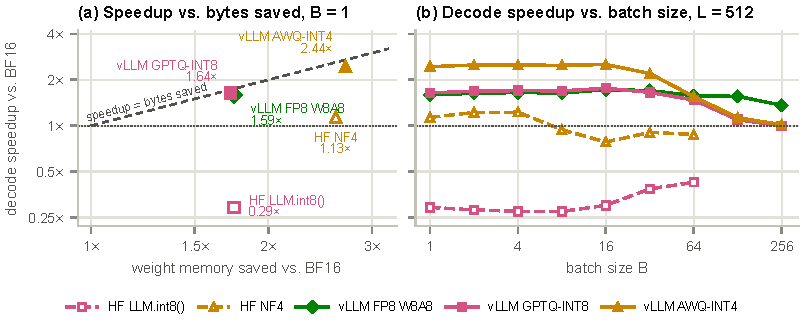
\includegraphics[width=\linewidth]{teaser_speedup}
\caption{\textbf{The bit-width does not predict the speedup.} (a)~Decode speedup over BF16 at batch
size~1 against the weight memory each format saves (Qwen2.5-7B, 512-token prompts). If decode time
were set only by the bytes read, every point would lie on the dashed line; the vLLM stack comes close,
the HF + bitsandbytes stack does not. (b)~As the batch grows, weight-only formats lose their gain; FP8 keeps it.}
\label{fig:teaser}
\end{figure}

\begin{itemize}
\item \textbf{Memory (Q1, \cref{sec:q1}).} 4-bit weights shrink Qwen2.5-7B by
  \WtNFSeven--\WtAWQSeven, not $4\times$, and the total saving drops to \MemBigNF{} with many tokens
  in flight. On vLLM the saved memory becomes KV cache (\KVratioAWQ{} more tokens).
\item \textbf{Speed (Q2, \cref{sec:q2}).} The implementation decides the speedup (\cref{fig:teaser}a): at
  batch size~1, vLLM's kernels turn \IdealAWQ--\IdealGQE\% of the byte saving into speed, NF4 only
  \IdealNF\%, and LLM.int8() is \INTeightslowdown{} slower than BF16.
\item \textbf{Crossover (Q3, \cref{sec:q3,sec:mechanism}).} Weight-only formats lose their speedup
  where decoding becomes compute-bound (\cref{fig:teaser}b; AWQ-INT4 at $B\approx\AWQcross$), while
  FP8 wins at every batch size. On HF, kernel launches on the CPU limit small models.
\item \textbf{Quality (Q4, \cref{sec:q4,sec:general}).} 8-bit formats stay within \EightKernMax{}
  points of BF16; 4-bit formats cost \MFourAbsMin--\MFourAbsMax{} MMLU points, more on smaller
  models, yet at a fixed memory budget a larger 4-bit model wins.
\end{itemize}

We release the harness, the raw data and the scripts that produce every number, table and figure in
this report.\footnote{\url{https://github.com/zz9tf/6359-SYS-ARCHITECT-course-work}}

\section{Background}
\label{sec:background}

\subsection{Two phases of LLM inference}
Autoregressive generation runs in two phases with very different hardware behavior.
In \emph{prefill}, all $L$ prompt tokens of each of the $B$ requests pass through the network at
once, so every linear layer is a GEMM with $M = B\cdot L$ rows. Its cost determines the
\emph{time to first token} (TTFT). In \emph{decode}, every step produces one new token per
request, so the same weights are multiplied by a matrix with only $M = B$ rows. Its cost per step
is the \emph{time per output token} (TPOT). The keys and values of all previous tokens are kept in
a KV cache whose size grows with $B\cdot(L+N)$ for $N$ generated tokens.

\subsection{A roofline view of quantization}
For a linear layer $y = xW^\top$ with $x\in\mathbb{R}^{M\times K}$ and $W\in\mathbb{R}^{N\times K}$
stored with $b$ bytes per weight, the arithmetic intensity is
\begin{equation}
  I(M) \;=\; \frac{2MNK}{b\,NK + 2MK + 2MN} \;\approx\; \frac{2M}{b}\quad (M \ll N, K).
  \label{eq:intensity}
\end{equation}
A kernel is memory-bound while $I(M)$ is below the GPU's ridge point
$P_{\text{peak}}/BW$ and compute-bound above it~\cite{williams2009roofline}. With BF16 weights
($b=2$), decode at small $B$ is deeply memory-bound: a step costs roughly the time needed to read
every weight once. Storing weights in 4 bits ($b\approx0.5$) cuts these bytes by about $4\times$,
which is the source of every decode-time speedup reported for weight-only quantization.
Three things work against it. (i) The weights must be dequantized back to 16 bits before the
tensor cores can use them, and this extra work is free only if a fused kernel hides it under the
memory stream. (ii) Weight-only formats (W4A16, W8A16) still compute in BF16, so once $I(M)$
reaches the ridge, at a $4\times$ smaller $M$ than BF16, the kernel is compute-bound and the
dequantization overhead is no longer hidden. (iii) Prefill is compute-bound from the start, so
weight-only formats cannot shorten TTFT. Formats that quantize the activations too (W8A8 in INT8
or FP8~\cite{micikevicius2022fp8}) also raise the compute ceiling, because the tensor cores run
8-bit math at twice the BF16 rate.

\subsection{Quantization methods studied}
\textbf{LLM.int8()}~\cite{dettmers2022llmint8} quantizes weights per output row and activations per
token to INT8. Activation feature columns that contain any value above a threshold (6.0) are
treated as outliers and multiplied in FP16 (mixed-precision decomposition).
\textbf{NF4}~\cite{dettmers2023qlora} stores weights in the 4-bit NormalFloat format with one
FP32 absmax scale per 64-weight block. Both are implemented in bitsandbytes and applied
to the BF16 checkpoint at load time through Hugging Face Transformers~\cite{hfbnb}.
\textbf{GPTQ}~\cite{frantar2023gptq} uses approximate second-order information to choose rounding
that minimizes each layer's output error. \textbf{AWQ}~\cite{lin2024awq} instead rescales the
weight channels that matter most for the activations before rounding. Both produce INT4 (or INT8)
weights with one FP16 scale per group of 128 weights, and are executed in vLLM~\cite{kwon2023vllm}
by the Marlin mixed-precision GEMM kernels~\cite{frantar2025marlin}. \textbf{FP8 W8A8} casts
the weights to E4M3 at load time with one scale per tensor and quantizes the activations
dynamically per token; vLLM runs it with CUTLASS FP8 GEMMs. SmoothQuant~\cite{xiao2023smoothquant} motivates the W8A8 design by moving
activation outliers into the weights; we use FP8 as its hardware-native counterpart on Blackwell.

\section{Experimental setup}
\label{sec:method}

\textbf{Platform.} We use one NVIDIA GeForce RTX 5090 (Blackwell, 170 SMs, 32\,GB GDDR7, 575\,W) in a
workstation with an Intel Core Ultra~9 285K and 64\,GB of RAM, running Ubuntu~24.04, PyTorch~2.13
(CUDA~13.0), Transformers~5.19, bitsandbytes~0.50.2 and vLLM~0.32 (CUDA graphs on). Our
microbenchmarks measure \BWmeas\,TB/s of memory bandwidth and \BFmeas{} (BF16) and \FPeightmeas{}
(FP8) TFLOP/s for large matrix multiplies, which puts the BF16 ridge point at about \RidgeBF{}
FLOP/byte.

\textbf{Models and configurations.} The main study uses instruction-tuned
Qwen2.5~\cite{qwen2024qwen25} at 3B, 7B and 14B parameters; Qwen3-8B and Qwen3-32B~\cite{qwen3} test
generality. \Cref{tab:configs} lists the eight configurations. The Hugging Face (HF) backend is what a
user gets with one extra argument to \texttt{from\_pretrained}: bitsandbytes quantizes the BF16
checkpoint while loading, and PyTorch runs the model eagerly. The vLLM backend serves the official
Qwen GPTQ and AWQ checkpoints with Marlin kernels and converts BF16 weights to FP8 while loading. The
embedding, the output layer (LM head) and the norms stay in 16 bits in every configuration.

\begin{table}[t]
\centering\small
\caption{The eight configurations. W/A: bits of the weights and of the activations in the matrix
multiply.}
\label{tab:configs}
\setlength{\tabcolsep}{4.5pt}
\begin{tabular}{llllll}
\toprule
Backend & Name & W/A & Method & Kernel & Weights from \\
\midrule
HF   & BF16      & 16/16           & ---            & cuBLAS                 & BF16 checkpoint \\
HF   & INT8      & 8/8$^{\dagger}$ & LLM.int8()     & bitsandbytes, cuBLASLt & quantized on load \\
HF   & NF4       & 4/16            & NF4, block 64  & bitsandbytes           & quantized on load \\
vLLM & BF16      & 16/16           & ---            & cuBLAS                 & BF16 checkpoint \\
vLLM & FP8       & 8/8             & FP8 E4M3       & CUTLASS                & quantized on load \\
vLLM & GPTQ-INT8 & 8/16            & GPTQ, group 128 & Marlin                & Qwen checkpoint \\
vLLM & AWQ-INT4  & 4/16            & AWQ, group 128  & Marlin                & Qwen checkpoint \\
vLLM & GPTQ-INT4 & 4/16            & GPTQ, group 128 & Marlin                & Qwen checkpoint \\
\bottomrule
\end{tabular}
\par\vspace{3pt}\parbox{\linewidth}{\scriptsize $^{\dagger}$Activation columns with values above 6.0
are multiplied in FP16.}
\end{table}

\textbf{Workloads.} \emph{Controlled sweep:} each configuration generates exactly 128 tokens for
$B\in\{1,2,4,\dots,64\}$ prompts (up to 256 on vLLM) of $L\in\{128,512,1024,2048\}$ random tokens,
so every configuration does the same work; a smaller sweep varies the output length. \emph{Real traffic:} 300 ShareGPT~\cite{sharegpt} conversations (median prompt 31 tokens,
median answer 284 tokens), served by vLLM to 1--64 concurrent clients and by HF in static batches of
16. \emph{Quality:} WikiText-2~\cite{merity2017wikitext} perplexity on 2048-token windows;
GSM8K~\cite{cobbe2021gsm8k} on all 1,319 test questions with zero-shot chain of thought and greedy
decoding; MMLU~\cite{hendrycks2021mmlu} on all 14,042 test questions, zero-shot. Prompts use each
model's chat template, and Qwen3 runs in non-thinking mode.

\textbf{Metrics and statistics.} TTFT is the time to the first output token, TPOT the mean time of
each later token, and throughput the number of output tokens per second. Each cell has one warm-up and
three measured runs with fresh prompts; the run-to-run variation of the end-to-end time is below
\CVmax\% in 95\% of the cells and \CVabsmax\% at most. Memory and energy come from PyTorch and NVML. For quality, all configurations answer the same
questions, so we compare each with HF BF16 by an exact McNemar test, with a Bonferroni correction over
the \MNumTests{} comparisons of each benchmark ($\alpha=\BonfAlpha$).

\section{Results}
\label{sec:results}

\subsection{Q1: How much memory does quantization actually save?}
\label{sec:q1}

\begin{figure}[t]
\centering
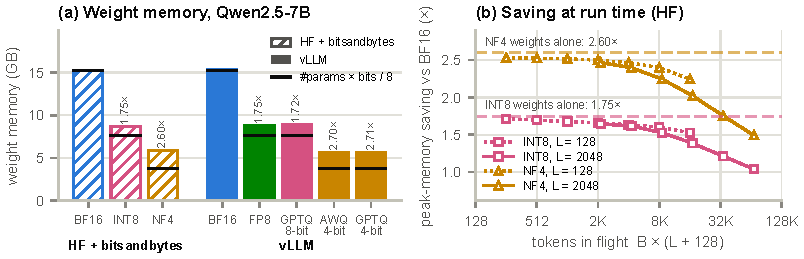
\includegraphics[width=\linewidth]{q1_memory_main}
\caption{\textbf{Q1: the real saving is smaller than the bit-width suggests.} (a)~Weight memory of
Qwen2.5-7B measured after loading (bars) against the naive estimate $\#\text{params}\times\text{bits}/8$
(black ticks); labels give the saving against BF16 on the same backend. (b)~Saving of the peak
memory on HF as more tokens are in flight (dashed: the saving of the weights alone).}
\label{fig:memory}
\end{figure}

\answer{Less than the bit-width suggests, and less as the context grows. On vLLM, the saved memory
becomes room for more requests.}

\textbf{Weights.} The naive estimate is too low for every format, by up to \NaiveExcessMax\% for NF4
(\cref{fig:memory}a). Only the decoder's linear layers are quantized: the embedding and the LM head
(\EmbedShareSeven\% of Qwen2.5-7B's parameters) stay in 16 bits, and each format stores scales.
Counting these parts predicts every HF measurement within \ModelErrMax\% (\cref{app:memory}). So
4-bit weights shrink the 7B model by \WtNFSeven{} (NF4) to \WtAWQSeven{} (AWQ-INT4), and 8-bit weights
by \WtIntEightSeven.

\textbf{Run time.} The KV cache and the activations are not quantized, so the saving shrinks as more
tokens are in flight (\cref{fig:memory}b). NF4 cuts the peak memory of one short request by
\MemSmallNF, but that of 32 requests of 2048 tokens by only \MemBigNF; LLM.int8(), which keeps extra
copies of the activations, by \MemBigInt. On HF, the 7B model runs out of memory at $B=64$, $L=2048$ in
every format, because the prefill activations fill the GPU.

\textbf{Capacity.} vLLM turns all the memory the weights leave free (within 85\% of the GPU) into KV
cache. With AWQ-INT4, Qwen2.5-7B holds \KVratioAWQ{} as many cached tokens as with BF16 (\KVawqSeven{}
vs.\ \KVbfSeven). \FourteenNote{}

\subsection{Q2: How do latency and throughput change?}
\label{sec:q2}

\begin{figure}[t]
\centering
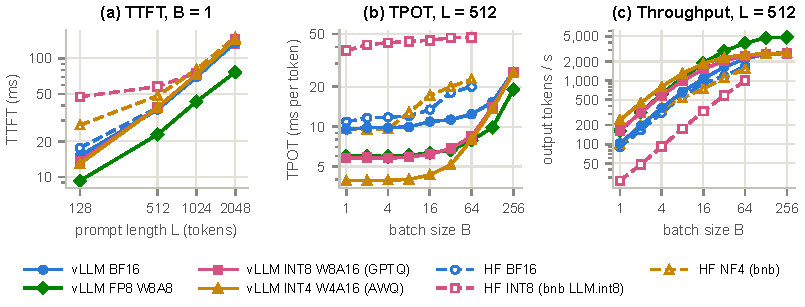
\includegraphics[width=\linewidth]{q2_latency_throughput}
\caption{\textbf{Q2: latency and throughput of Qwen2.5-7B} with 128 generated tokens. (a)~TTFT of one
request; (b)~TPOT and (c)~output throughput for 512-token prompts. Solid lines: vLLM; dashed lines
with hollow markers: HF with bitsandbytes.}
\label{fig:latency}
\end{figure}

\answer{With fused kernels, fewer bytes give an almost proportional decode speedup for small
batches; with bitsandbytes they do not. No weight-only format shortens prefill.}

\textbf{Decode.} At batch size 1 (prediction P1), vLLM's BF16 step takes \TPOTbfVllmSeven\,ms,
within \BWutilVllm\% of the time needed to read the 15.2\,GB of weights, so it is purely memory-bound.
On vLLM, fewer bytes do mean less time (\cref{fig:latency}b): AWQ-INT4 decodes \AWQspeedup{} faster
than BF16, GPTQ-INT8 \GPTQeightspeedup{} and FP8 \FPeightspeedup, which is \IdealAWQ--\IdealGQE\% of
their byte savings. On HF the same idea fails: LLM.int8() is \INTeightslowdown{} slower than BF16, and
NF4 is \NFsevenB{} faster on 7B (\NFfourteenB{} on 14B) but \NFthreeslow{} slower on 3B.
These are whole stacks: LLM.int8() and GPTQ-INT8 differ in method, activation path and engine, not
only in kernel. \Cref{sec:mechanism} separates the kernels from the rest.

\textbf{Prefill.} As P3 predicts, AWQ and GPTQ change the TTFT by at most \TTFTwoMax\%, and NF4 makes
it \TTFTnfSlow{} slower, because bitsandbytes dequantizes every weight matrix first
(\cref{fig:latency}a). FP8, which also quantizes the activations, makes a 2048-token prefill
\TTFTfpLong{} faster.

\textbf{Throughput.} At $B=256$ (\cref{fig:latency}c), AWQ-INT4 (\ThrAWQmax{} tokens/s) no longer
beats BF16 (\ThrBFmax), while FP8 reaches \ThrFPmax{} tokens/s, \ThrFPratio{} the BF16 rate. Energy
per token follows latency (\cref{app:speed}).

\subsection{Q3: When does lower precision pay off?}
\label{sec:q3}

\begin{figure}[t]
\centering
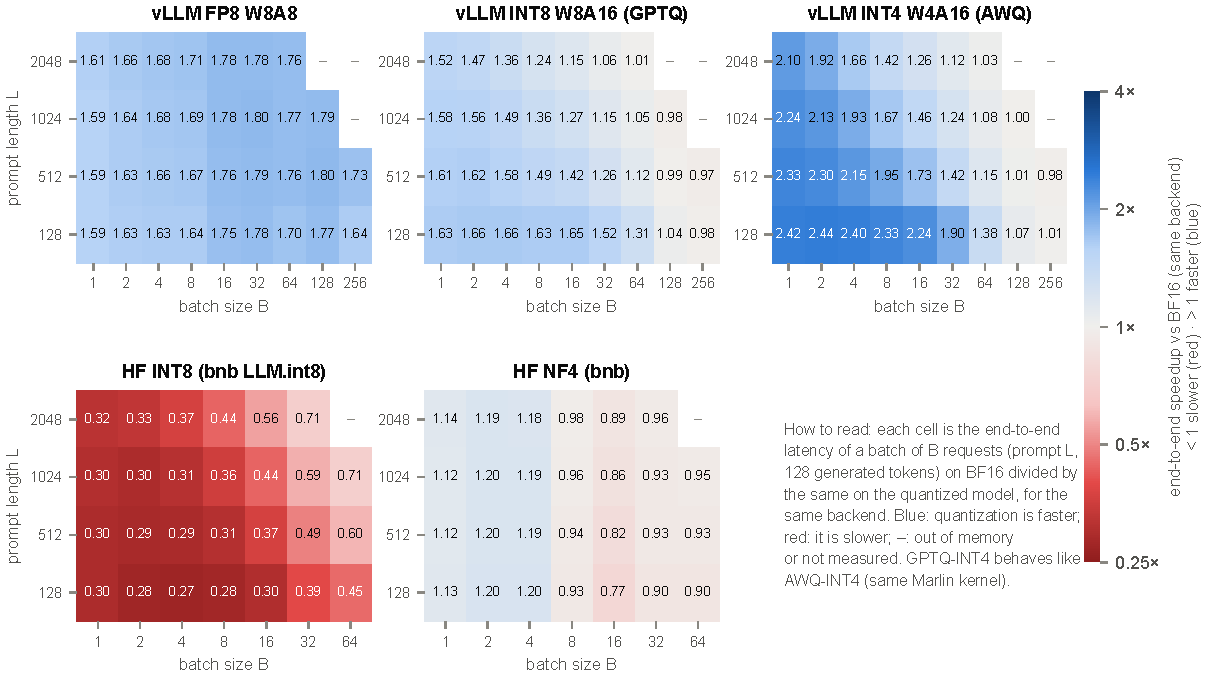
\includegraphics[width=\linewidth]{q3_speedup_heatmaps}
\caption{\textbf{Q3: where each format pays off.} End-to-end speedup of $B$ requests ($L$-token prompts,
128 generated tokens) over BF16 on the same backend, Qwen2.5-7B. Dashes: out of memory or not run.
GPTQ-INT4 behaves like AWQ-INT4 (\cref{tab:crossover} in \cref{app:speed}).}
\label{fig:heatmaps}
\end{figure}

\answer{Weight-only formats pay off for small batches, and their gain ends near the batch size at
which decoding becomes compute-bound. FP8 pays off everywhere; the bitsandbytes formats rarely do.}

\Cref{fig:heatmaps} maps the end-to-end speedup over batch size and prompt length. Three regimes
appear. (i)~\emph{Weight-only formats with fused kernels} (AWQ, GPTQ) win by up to \AWQmaxEtoE{} when
decode dominates. Their gain shrinks as the batch and the prompts grow, and AWQ-INT4 stops winning at
$B\approx\AWQcross$ for 512-token prompts, close to $M\approx R\approx\RidgeBF$, where BF16 decoding
itself becomes compute-bound (P2).
(ii)~\emph{FP8 W8A8} wins in every cell (\FPminEtoE--\FPmaxEtoE), because it halves the bytes
\emph{and} raises the compute roof. (iii)~\emph{bitsandbytes formats} rarely win: LLM.int8() is slower
in every cell (\INTminEtoE--\INTmaxEtoE), and NF4 wins only for 7B below $B\approx\NFcross$. Longer
answers raise the share of decode and push the crossover up: at $B=16$, AWQ-INT4 speeds up a request
with 32 output tokens by \OutAWQSixteenShort, but one with 512 output tokens by \OutAWQSixteenLong{}
(\cref{app:speed}).

\subsection{Why: kernels, the roofline and host overhead}
\label{sec:mechanism}

\begin{figure}[t]
\centering
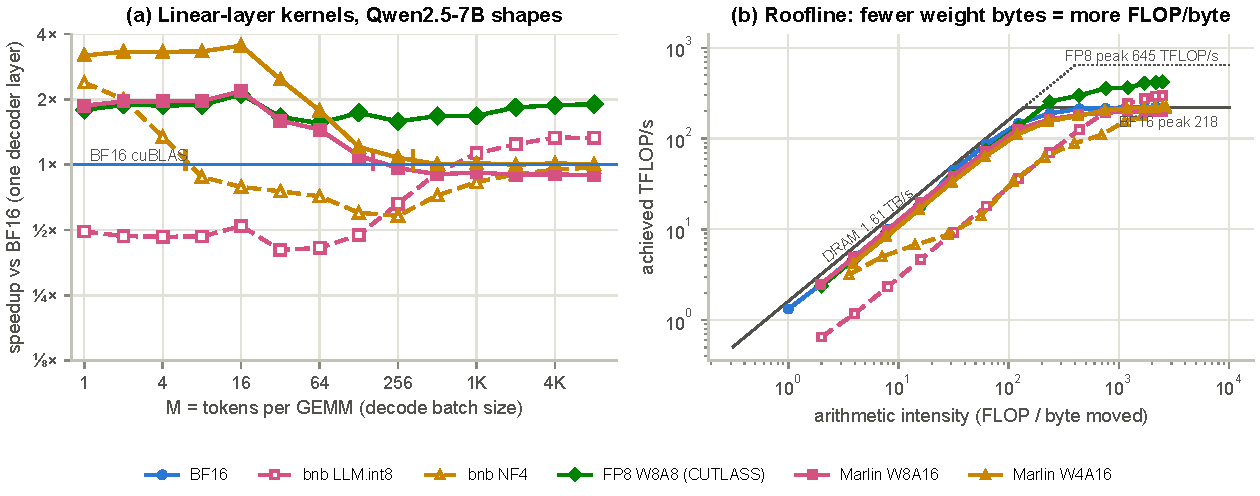
\includegraphics[width=\linewidth]{q3_kernel_crossover}
\caption{\textbf{Why the crossover happens.} (a)~Speedup of each low-bit kernel over BF16 cuBLAS on the
matrix shapes of one Qwen2.5-7B decoder layer, against the tokens $M$ per multiply (the decode batch
size); ticks mark where it falls below 1.05. (b)~The same kernels on the measured roofline.}
\label{fig:kernels}
\end{figure}

\answer{The roofline explains vLLM, where the kernels are fast. The CPU cost of launching kernels
explains HF, where the GPU is often idle.}

\textbf{Kernels.} We time each low-bit kernel alone on the matrix shapes of one 7B decoder layer
(\cref{fig:kernels}a). Marlin W4A16 is \MarlinFourMone{} faster than BF16 at $M=1$ and keeps a gain
above 5\% up to $M\approx\MarlinFourCross$; Marlin W8A16 starts at \MarlinEightMone{} and ends at
$M\approx\MarlinEightCross$. \Cref{fig:kernels}b shows why (P2): fewer bytes per weight move a kernel
up the bandwidth roof faster, but it hits the same BF16 compute roof. Real kernels approach the roof
gradually, so the crossovers lie somewhat above the ridge point. FP8 W8A8 is \FPkernMone{} faster at
$M=1$ and still \FPkernMmax{} at $M=8192$, because its compute roof is about three times higher
(\FPeightmeas{} vs.\ \BFmeas\,TFLOP/s). The bitsandbytes kernels are not slow everywhere: NF4's
kernel is \NFkernMone{} faster than BF16 at $M=1$ (it dequantizes whole matrices for larger $M$), yet
the whole NF4 model is only \NFsevenB{} faster. Time must be lost outside the kernels.

\begin{figure}[t]
\centering
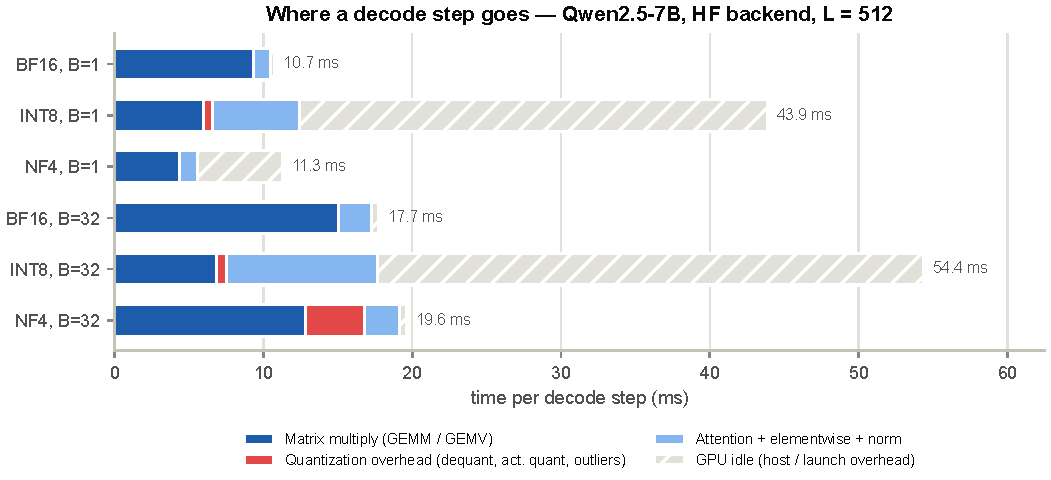
\includegraphics[width=\linewidth]{mech_decode_breakdown}
\caption{\textbf{Where an HF decode step goes} (Qwen2.5-7B, 512-token prompts): GPU time by kernel
type, and the time the GPU waits for the CPU (hatched).}
\label{fig:profile}
\end{figure}

\textbf{Host overhead.} \Cref{fig:profile} profiles one HF decode step of the 7B model. With BF16, the
GPU is busy \BusyBFone\% of the step. LLM.int8() launches \KernIntRatio{} as many kernels (casts,
outlier handling, quantization, two matrix multiplies per layer), and the GPU is busy only
\BusyIntone\% of the time: Python and kernel launches set the speed. NF4 lies in between (\BusyNFone\%
busy). More layers mean more launches, so the 36-layer 3B model suffers more than the 28-layer 7B
model. vLLM avoids most of this cost with CUDA graphs, which replay a decode step with very few launches.

\subsection{Do the results hold for real traffic?}
\label{sec:real}
\answer{Yes, and the serving system matters even more than the number format.}
In a replay of 300 ShareGPT requests (\cref{tab:serving_main} in \cref{app:real}), AWQ-INT4 gives the lowest TPOT with
one client (\SrvTPOTawqOne\,ms vs.\ \SrvTPOTbfOne\,ms for BF16), and FP8 the highest throughput with 64
clients (\SrvThrFP{} vs.\ \SrvThrBF{} tokens/s), as the crossover of \cref{sec:q3} predicts. With the
same 16 requests in flight, vLLM BF16 delivers \SrvGap{} the throughput of HF BF16. Both run BF16, so
this gap belongs to the serving stack (continuous~\cite{yu2022orca} vs.\ static batching, CUDA
graphs), not to quantization; the two stacks are also timed differently (\cref{app:real}).



\subsection{Q4: How much quality does quantization cost?}
\label{sec:q4}
\Cref{tab:quality,fig:quality} report WikiText-2 perplexity and GSM8K accuracy. Every GSM8K
comparison is paired: all configurations answer the same 1,319 questions, so we test each
difference against HF BF16 with an exact McNemar test on the questions where exactly one of the two
runs is correct.

\textbf{Noise floor.} Even two BF16 runs of the same weights disagree. vLLM and HF use different
kernels and accumulation orders, and greedy decoding turns the resulting rounding differences into
different reasoning chains: the two backends disagree on \BackendFlipsSeven{} of the 7B model's
questions and their accuracies differ by \BackendNoiseSeven{} points (\BackendNoiseThree{} for 3B).
Differences of this size are not caused by quantization.

\textbf{8-bit formats preserve quality.} LLM.int8(), GPTQ-INT8 and FP8 W8A8 stay within
\DEightAbsSeven{} GSM8K points and \PPLEightAbsSeven{} perplexity of BF16 on the 7B model
(\DEightAbsThree{} points on 3B), and \EightSentence.

\textbf{4-bit formats cost little on 7B and more on 3B.} The 4-bit formats raise perplexity by
\PPLFourMinSeven{} to \PPLFourMaxSeven{} on the 7B model, and its GSM8K accuracy changes by only
\DFourMinSeven{} to \DFourMaxSeven{} points, none significant. The 3B model loses
\DFourMinThree{} to \DFourMaxThree{} points with \PPLFourMinThree{} to \PPLFourMaxThree{}
perplexity, and \FourThreeSurvive{} of these drops remain significant after a Bonferroni correction:
a smaller model has less redundancy to absorb the rounding error.

\textbf{Model size versus bit-width.} \Cref{fig:quality} places every configuration by its weight
memory. \QualityGuide{} At a fixed memory budget, parameters are worth more than bits.

\textbf{One metric is not enough.} The 14B GPTQ-INT4 checkpoint scores \AccGPTQFourFourteenPct\%
on GSM8K, on par with the other 14B formats, yet its WikiText-2 perplexity is
\PPLGPTQFourFourteen{} against \PPLOthersFourteen{} for AWQ-INT4, GPTQ-INT8 and FP8. The outlier
is not an artifact of our setup: it persists with BF16 instead of FP16 activations, the loss is
elevated at every position of the 2048-token window, and the same harness scores the 7B GPTQ-INT4
checkpoint normally. Ranking the next token shows what happened. On raw WikiText the checkpoint predicts the
next token correctly only \TopOneGPTQWiki\% of the time (\TopOneOthersWiki\% for the other 14B
formats), whereas on chat-formatted GSM8K solutions it matches them (\TopOneGPTQChat\% vs.\
\TopOneOthersChat\%). The quantized weights still model the chat distribution they serve but have
lost much of their general language modeling. GSM8K alone would have missed this; perplexity alone
would have rejected a checkpoint that works for chat.

\begin{table}[t]
\centering
\footnotesize
\caption{Q4 --- quality. WikiText-2 perplexity (2048-token windows) and GSM8K accuracy (1,319 questions, zero-shot CoT, greedy decoding). Deltas are against HF BF16 of the same model; $p$ is the two-sided exact McNemar test of the paired GSM8K answers against HF BF16.}
\label{tab:quality}
\setlength{\tabcolsep}{3.2pt}
\begin{tabular}{llrrrrr}
\toprule
Model & Config & PPL & $\Delta$PPL & GSM8K (\%) & $\Delta$acc & $p$ \\
\midrule
3B & HF BF16 & 8.56 & -- & 85.8 & -- & -- \\
 & HF INT8 & 8.66 & $+0.10$ & 85.5 & $-0.3$ & 0.777 \\
 & HF NF4 & 9.11 & $+0.55$ & 82.6 & $-3.3$ & $<$0.001 \\
 & vLLM BF16 & 8.56 & $+0.00$ & 86.0 & $+0.2$ & 0.871 \\
 & vLLM FP8 & 8.64 & $+0.09$ & 85.4 & $-0.5$ & 0.610 \\
 & vLLM GPTQ-8 & 8.56 & $+0.00$ & 86.4 & $+0.6$ & 0.322 \\
 & vLLM AWQ-4 & 9.10 & $+0.54$ & 82.7 & $-3.1$ & 0.002 \\
 & vLLM GPTQ-4 & 9.22 & $+0.66$ & 82.0 & $-3.8$ & $<$0.001 \\
7B & HF BF16 & 7.46 & -- & 90.8 & -- & -- \\
 & HF INT8 & 7.49 & $+0.03$ & -- & -- & -- \\
 & HF NF4 & 7.77 & $+0.31$ & 90.3 & $-0.5$ & 0.500 \\
 & vLLM BF16 & 7.46 & $+0.00$ & 91.2 & $+0.4$ & 0.359 \\
 & vLLM FP8 & 7.51 & $+0.05$ & 90.8 & $+0.0$ & 1.000 \\
 & vLLM GPTQ-8 & 7.46 & $+0.00$ & 91.7 & $+0.9$ & 0.043 \\
 & vLLM AWQ-4 & 7.85 & $+0.39$ & 90.4 & $-0.5$ & 0.576 \\
 & vLLM GPTQ-4 & 7.78 & $+0.32$ & 91.1 & $+0.2$ & 0.828 \\
14B & vLLM FP8 & 5.77 & -- & 94.4 & -- & -- \\
 & vLLM GPTQ-8 & 5.71 & -- & 94.7 & -- & -- \\
 & vLLM AWQ-4 & 6.16 & -- & 93.9 & -- & -- \\
 & vLLM GPTQ-4 & 37.46$^{\ddagger}$ & -- & 93.7 & -- & -- \\
\bottomrule
\end{tabular}
\par\vspace{2pt}\parbox{\linewidth}{\scriptsize $^{\ddagger}$Degraded on raw text but not on chat-formatted text; see \cref{sec:q4}.}
\end{table}



\subsection{Do the results generalize? Qwen3-8B and Qwen3-32B}
\label{sec:general}
To check that the conclusions are not specific to Qwen2.5, we repeated the core measurements on
Qwen3-8B~\cite{qwen3}, a newer model with a different layout (\FamRLayers{} layers and \FamRKVheads{}
KV heads against \FamQLayers{} and \FamQKVheads{} for Qwen2.5-7B), run in non-thinking mode.
\Cref{tab:general} compares the two on the same grid.

The systems results carry over almost unchanged. 4-bit weights shrink by \FamRAWQsave{} rather than
$4\times$; at batch size one AWQ-INT4 decodes \FamRAWQone{} faster (\FamQAWQone{} for Qwen2.5-7B),
FP8 \FamRFPone{} faster, and LLM.int8() runs at \FamRINTone{} of the BF16 speed. At $B=\FamRBcmp$
FP8 still raises throughput by \FamRFPthr{} while AWQ-INT4 has fallen to \FamRAWQthr. The one
difference confirms the host-overhead explanation of \cref{sec:mechanism}: NF4, \FamQNFone{} faster
than BF16 on the 28-layer Qwen2.5-7B, is \FamRNFone{} on the 36-layer Qwen3-8B, just as it was
slower on the 36-layer Qwen2.5-3B. More layers mean more kernel launches per decode step, and the
step becomes bound by the host rather than by memory. Qwen3-8B also stores \FamKVratio{} as many
KV-cache bytes per token, so at $B=256$ none of its configurations fits the cache; the memory a
format saves on weights matters even more for such models. \FamQualitySentence

\textbf{Scaling up: Qwen3-32B.} At 32B parameters the question changes from speed to feasibility.
Qwen3-32B needs \BigBFw\,GB in BF16 and about half of that in FP8 or INT8, more than the GPU's
32\,GB, so on this GPU it runs only at 4 bits: AWQ-INT4 takes \BigAWQw\,GB and leaves room for
\BigAWQkv{} cached tokens, and NF4 takes \BigNFw\,GB. Against Qwen3-8B in BF16 (\SmallBFw\,GB, a
similar budget), the 4-bit 32B model needs \BigAWQtpot\,ms per decoded token at batch size one
(vLLM; 8B BF16: \SmallBFtpot\,ms) and scores \BigGSMawq\% vs.\ \SmallGSMbf\% on GSM8K
(\BigGAWQp) and \BigMMLUawq\% vs.\ \SmallMMLUbf\% on MMLU (\BigMAWQp). \BigVerdict{} One caveat is
numerical: the AWQ checkpoint ships FP16 activations, and in \BigNaNwin{} perplexity windows the
activations overflow beyond the first 512 positions and the loss becomes NaN; with BF16
activations every window is finite (perplexity \BigPPLawq), so long-context use of this
checkpoint should run in BF16.

\begin{table}[htbp]
\centering
\small
\caption{The main results for Qwen2.5-7B and Qwen3-8B (non-thinking mode) on the same grid (512-token prompts, 128 output tokens). Throughput is compared at the largest batch at which both models' KV caches hold every request ($B=64$). Qwen3-8B has no official GPTQ checkpoint.}
\label{tab:general}
\setlength{\tabcolsep}{3.2pt}
\begin{tabular}{lrr}
\toprule
Metric (vs.\ BF16) & Qwen2.5-7B & Qwen3-8B \\
\midrule
Weight saving, AWQ-INT4 (vLLM) & 2.70$\times$ & 2.67$\times$ \\
Weight saving, NF4 (HF) & 2.60$\times$ & 2.55$\times$ \\
Decode speedup $B=1$, AWQ-INT4 & 2.44$\times$ & 2.33$\times$ \\
Decode speedup $B=1$, FP8 & 1.59$\times$ & 1.54$\times$ \\
Decode speedup $B=1$, NF4 & 1.13$\times$ & 0.90$\times$ \\
Decode speedup $B=1$, LLM.int8() & 0.29$\times$ & 0.28$\times$ \\
Throughput $B=64$, AWQ-INT4 & 1.15$\times$ & 1.12$\times$ \\
Throughput $B=64$, FP8 & 1.76$\times$ & 1.67$\times$ \\
GSM8K $\Delta$ pp ($p$), FP8 & $0.0$ (1.000) & $+0.5$ (0.488) \\
GSM8K $\Delta$ pp ($p$), LLM.int8() & $-0.2$ (0.771) & $+0.6$ (0.382) \\
GSM8K $\Delta$ pp ($p$), AWQ-INT4 & $-0.5$ (0.576) & $-0.2$ (0.818) \\
GSM8K $\Delta$ pp ($p$), NF4 & $-0.5$ (0.500) & $+0.2$ (0.909) \\
MMLU $\Delta$ pp ($p$), FP8 & $-0.1$ (0.327) & $-0.7$ ($<$0.001) \\
MMLU $\Delta$ pp ($p$), LLM.int8() & $-0.2$ (0.134) & $+0.7$ ($<$0.001) \\
MMLU $\Delta$ pp ($p$), AWQ-INT4 & $-1.6$ ($<$0.001) & $-0.7$ (0.003) \\
MMLU $\Delta$ pp ($p$), NF4 & $-0.6$ (0.002) & $-0.3$ (0.156) \\
\bottomrule
\end{tabular}
\end{table}



\section{Discussion}
\label{sec:discussion}

\subsection{When does quantization pay off?}
Our measurements reduce to five rules for deploying a quantized LLM on a GPU like the RTX 5090.

\textbf{(1) Budget memory with the real ratio, not $16/b$.} Every format saves memory, but the
16-bit embedding, LM head and scales cap 4-bit formats at \WtNFSeven--\WtAWQSeven{} for a 7B
model, and the KV cache and activations are not quantized at all. A capacity plan that assumes
$4\times$ will run out of memory.

\textbf{(2) For interactive, low-concurrency serving, use 4-bit weight-only formats with fused
kernels.} At one request per GPU, AWQ-INT4 with Marlin decodes \AWQspeedup{} faster than BF16
and uses \EnRatioAWQone{} less energy per token.

\textbf{(3) For high-throughput serving, use W8A8 FP8.} Weight-only formats lose their advantage
once the batch makes decode compute-bound ($B\gtrsim\AWQcross$ for AWQ at 512-token prompts) and
never speed up prefill. FP8 is the only format that keeps winning, with \ThrFPratio{} the BF16
throughput at $B=256$, because it also doubles the tensor-core rate.

\textbf{(4) Quantize for memory, not speed, when only bitsandbytes is available.} LLM.int8() is
\INTeightslowdown{} slower than BF16 at batch size one and never catches up, and NF4 is faster only
for small batches of a model large enough to be memory-bound. Both remain useful to fit a model
that otherwise would not fit.

\textbf{(5) \GuideHead} \QualityGuide

\noindent Across all five, the bit-width alone predicts very little; the kernel that executes the
format and the regime the workload puts the GPU in decide the outcome.

\textbf{Limitations.} We test one GPU and dense Qwen models. The mechanism is architectural and Qwen3
reproduces it, but crossover batch sizes depend on each GPU's ratio of compute to bandwidth. The GPU
also drives a display, so we could not lock its clocks (repeated runs still agree closely). We do not
study 4-bit activations, KV-cache quantization or mixture-of-experts models.
\label{sec:limits}


\section{Conclusion}
\label{sec:conclusion}
We measured how much memory LLM quantization saves and when it makes inference faster, using
eight configurations of Qwen2.5 models on an RTX 5090. Memory savings are real but smaller than
advertised: \WtNFSeven{} instead of $4\times$ for 4-bit weights, and as little as \MemBigNF{} end
to end once the KV cache grows. Speed depends on the kernel and the regime rather than on the
bit-width: the same 8-bit weights decode \GPTQeightspeedup{} faster than BF16 with Marlin and
\INTeightslowdown{} slower with bitsandbytes, weight-only gains disappear in the compute-bound regime, and FP8 W8A8 is the only
format that is faster everywhere. \QualityConclusion{} Smaller is not always faster---but with the
right kernel, for the right regime, it is both smaller and faster.

\section*{Division of work}
Following the proposal, Sijia Zhong built the baseline harness and the memory study (Q1), Zheng Zheng
ran the controlled precision/batch/length sweeps and the kernel and profiling analysis (Q2), and
Haofei Sun ran the ShareGPT and quality evaluations (Q3, Q4). All three analyzed the results and
wrote the report and slides.


\balance
\bibliographystyle{IEEEtran}
\bibliography{refs}

\section{Additional memory results}
\label{app:memory}

\Cref{fig:weights,tab:weights} give the weight memory of every configuration and model size.
\Cref{fig:breakdown} splits the peak memory of the 7B model on HF into weights, KV cache and
activations. It shows why the run-time saving shrinks: as the batch grows, the KV cache and the
activations take a growing share of the peak memory, and neither is quantized. \Cref{fig:kvcap} shows the
KV-cache capacity that vLLM gets from the memory each format frees.

\begin{figure}[htbp]
\centering
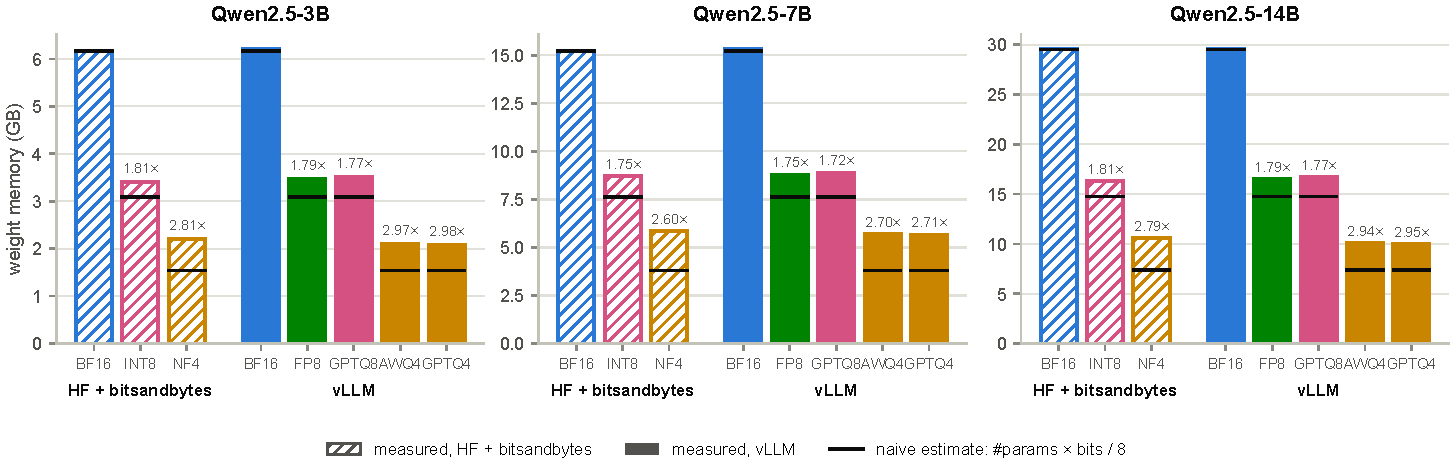
\includegraphics[width=\linewidth]{q1_weight_memory}
\caption{Weight memory of every configuration for the three Qwen2.5 sizes (bars: measured; black
ticks: $\#\text{params}\times\text{bits}/8$). Labels give the saving against BF16 on the same backend.}
\label{fig:weights}
\end{figure}

\begin{table*}[t]
\centering
\footnotesize
\caption{Q1 --- weight memory: naive estimate ($\#$params$\times$bits/8), our analytic model (unquantized embedding/LM head/norms + quantization metadata), and measured on the GPU.}
\label{tab:weights}
\setlength{\tabcolsep}{4pt}
\begin{tabular}{llrrrrr}
\toprule
Model & Config & Naive (GB) & Model (GB) & Measured (GB) & Ratio vs BF16 & Naive ratio \\
\midrule
Qwen2.5-7B & HF BF16 & 15.23 & 15.23 & 15.23 & 1.00$\times$ & 1.00$\times$ \\
Qwen2.5-7B & HF INT8 (LLM.int8) & 7.62 & 8.71 & 8.71 & 1.75$\times$ & 2.00$\times$ \\
Qwen2.5-7B & HF NF4 & 3.81 & 5.85 & 5.85 & 2.60$\times$ & 4.00$\times$ \\
Qwen2.5-7B & vLLM BF16 & 15.23 & 15.23 & 15.34 & 1.00$\times$ & 1.00$\times$ \\
Qwen2.5-7B & vLLM FP8 W8A8 & 7.62 & 8.71 & 8.77 & 1.75$\times$ & 2.00$\times$ \\
Qwen2.5-7B & vLLM GPTQ W8A16 & 7.62 & 8.86 & 8.90 & 1.72$\times$ & 2.00$\times$ \\
Qwen2.5-7B & vLLM AWQ W4A16 & 3.81 & 5.57 & 5.68 & 2.70$\times$ & 4.00$\times$ \\
Qwen2.5-7B & vLLM GPTQ W4A16 & 3.81 & 5.57 & 5.66 & 2.71$\times$ & 4.00$\times$ \\
Qwen2.5-14B & HF BF16 & 29.54 & 29.54 & 29.54 & 1.00$\times$ & 1.00$\times$ \\
Qwen2.5-14B & HF INT8 (LLM.int8) & 14.77 & 16.33 & 16.34 & 1.81$\times$ & 2.00$\times$ \\
Qwen2.5-14B & HF NF4 & 7.39 & 10.55 & 10.58 & 2.79$\times$ & 4.00$\times$ \\
Qwen2.5-14B & vLLM BF16 & 29.54 & 29.54 & 29.60 & 1.00$\times$ & 1.00$\times$ \\
Qwen2.5-14B & vLLM FP8 W8A8 & 14.77 & 16.33 & 16.51 & 1.79$\times$ & 2.00$\times$ \\
Qwen2.5-14B & vLLM GPTQ W8A16 & 14.77 & 16.64 & 16.73 & 1.77$\times$ & 2.00$\times$ \\
Qwen2.5-14B & vLLM AWQ W4A16 & 7.39 & 9.98 & 10.07 & 2.94$\times$ & 4.00$\times$ \\
Qwen2.5-14B & vLLM GPTQ W4A16 & 7.39 & 9.98 & 10.02 & 2.95$\times$ & 4.00$\times$ \\
\bottomrule
\end{tabular}
\end{table*}


\begin{figure}[htbp]
\centering
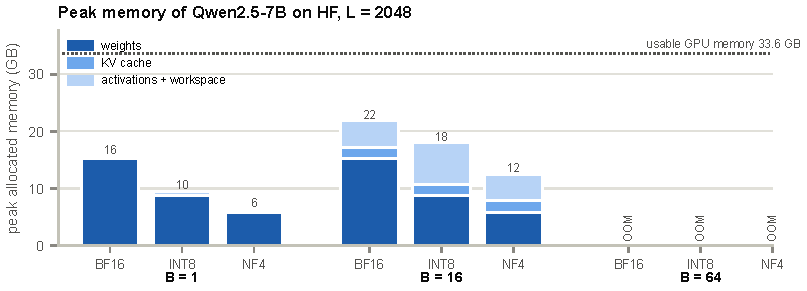
\includegraphics[width=\linewidth]{q1_memory_breakdown}
\caption{Peak allocated memory of Qwen2.5-7B on HF with 2048-token prompts, split into weights, KV
cache and activations. OOM: out of memory.}
\label{fig:breakdown}
\end{figure}

\begin{figure}[htbp]
\centering
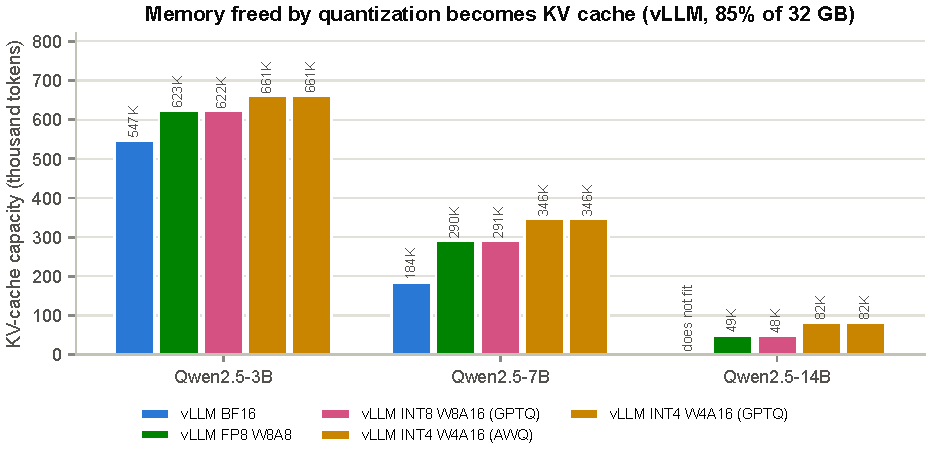
\includegraphics[width=\linewidth]{q1_kv_capacity}
\caption{KV-cache capacity that vLLM allocates with 85\% of the GPU after loading the weights.}
\label{fig:kvcap}
\end{figure}

\FloatBarrier
\section{Additional speed results}
\label{app:speed}

\Cref{tab:speed} lists the latency, throughput and energy numbers behind \cref{fig:latency}, and
\cref{tab:crossover} lists where each format stops paying off (\cref{fig:heatmaps}).
\Cref{fig:energy} shows the energy per output token. GPU power stays close to the board limit in
every configuration (\PowerRange\,W), so energy per token follows latency. LLM.int8() draws little
power (\PowerInt\,W) but runs so long that it uses the most energy per token. \Cref{fig:outlen}
shows how the answer length moves the speedup (\cref{sec:q3}).

\begin{table}[htbp]
\centering
\footnotesize
\caption{Latency, throughput and energy of Qwen2.5-7B with 512-token prompts and 128 output tokens (mean of 3 runs). Subscripts give the batch size. TTFT and TPOT in ms; Speedup$_1$ is the decode speedup over BF16 on the same backend; energy is GPU energy per output token.}
\label{tab:speed}
\setlength{\tabcolsep}{4pt}
\begin{tabular}{lrrrrrrr}
\toprule
Config & TTFT$_{1}$ & TPOT$_{1}$ & TPOT$_{64}$ & tok/s$_{64}$ & Speedup$_{1}$ & mJ/tok$_{1}$ & mJ/tok$_{64}$ \\
\midrule
HF BF16 & 38.4 & 10.90 & 20.04 & 1669 & 1.00$\times$ & 5092 & 294 \\
HF INT8 (LLM.int8) & 57.8 & 37.45 & 47.14 & 1003 & 0.29$\times$ & 6187 & 305 \\
HF NF4 & 48.3 & 9.62 & 22.87 & 1550 & 1.13$\times$ & 3188 & 340 \\
vLLM BF16 & 37.0 & 9.52 & 12.39 & 2209 & 1.00$\times$ & 4878 & 249 \\
vLLM FP8 W8A8 & 22.8 & 5.99 & 7.88 & 3886 & 1.59$\times$ & 2507 & 141 \\
vLLM GPTQ W8A16 & 38.5 & 5.80 & 8.41 & 2471 & 1.64$\times$ & 2588 & 234 \\
vLLM AWQ W4A16 & 38.6 & 3.90 & 7.99 & 2544 & 2.44$\times$ & 1919 & 224 \\
vLLM GPTQ W4A16 & 36.9 & 3.88 & 7.89 & 2642 & 2.45$\times$ & 1840 & 219 \\
\bottomrule
\end{tabular}
\end{table}

\begin{table}[htbp]
\centering
\footnotesize
\caption{Where each format stops paying off (Qwen2.5-7B, 512-token prompts, 128 output tokens). Speedup over BF16 on the same backend at batch size 1 and at the largest batch we ran (in brackets), and the batch size up to which the format is faster (linear interpolation in $\log B$).}
\label{tab:crossover}
\setlength{\tabcolsep}{3.5pt}
\begin{tabular}{lrrlrrl}
\toprule
 & \multicolumn{3}{c}{Decode step (TPOT)} & \multicolumn{3}{c}{Whole request (E2E)} \\
\cmidrule(lr){2-4}\cmidrule(lr){5-7}
Config & $B{=}1$ & largest $B$ & faster up to & $B{=}1$ & largest $B$ & faster up to \\
\midrule
HF INT8 (LLM.int8) & 0.29$\times$ & 0.43$\times$ (64) & never & 0.30$\times$ & 0.60$\times$ (64) & never \\
HF NF4 & 1.13$\times$ & 0.88$\times$ (64) & $B\approx7$ & 1.12$\times$ & 0.93$\times$ (64) & $B\approx7$ \\
vLLM FP8 W8A8 & 1.59$\times$ & 1.36$\times$ (256) & all $B$ & 1.59$\times$ & 1.73$\times$ (256) & all $B$ \\
vLLM GPTQ W8A16 & 1.64$\times$ & 1.00$\times$ (256) & $B\approx251$ & 1.61$\times$ & 0.97$\times$ (256) & $B\approx123$ \\
vLLM AWQ W4A16 & 2.44$\times$ & 1.02$\times$ (256) & all $B$ & 2.33$\times$ & 0.98$\times$ (256) & $B\approx175$ \\
vLLM GPTQ W4A16 & 2.45$\times$ & 1.05$\times$ (256) & all $B$ & 2.35$\times$ & 1.03$\times$ (256) & all $B$ \\
\bottomrule
\end{tabular}
\end{table}


\begin{figure}[htbp]
\centering
\begin{minipage}[t]{0.46\linewidth}
\centering
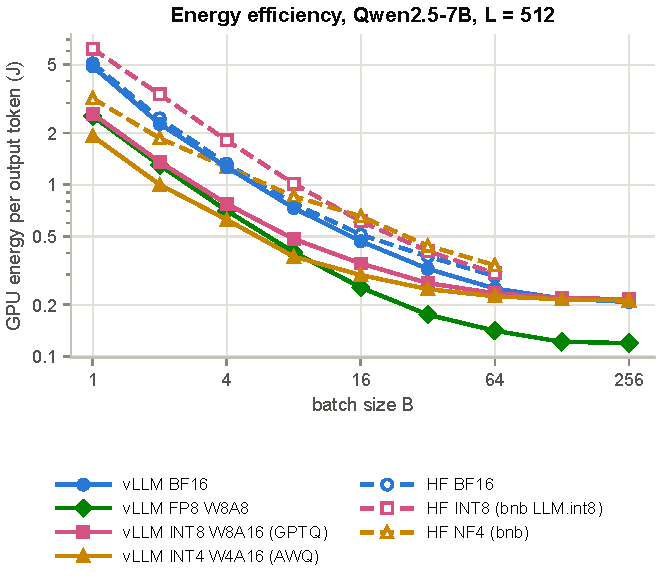
\includegraphics[width=\linewidth]{energy_per_token}
\caption{GPU energy per output token (NVML), Qwen2.5-7B, 512-token prompts.}
\label{fig:energy}
\end{minipage}\hfill
\begin{minipage}[t]{0.5\linewidth}
\centering
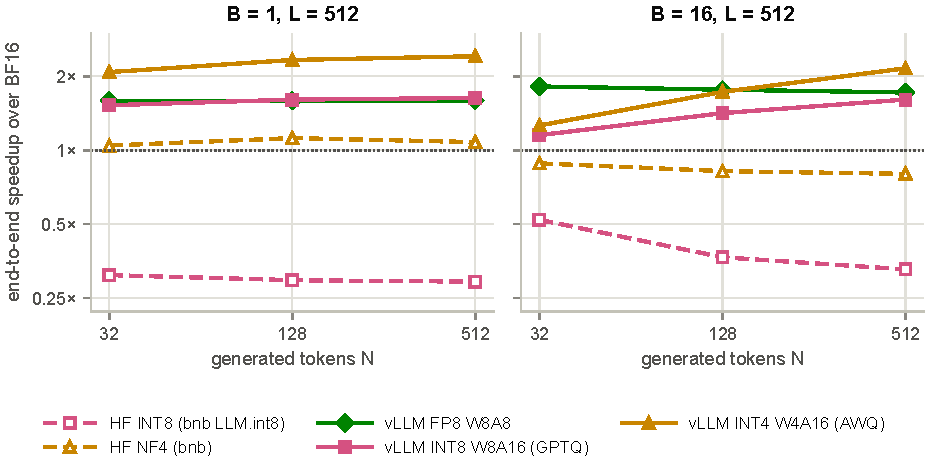
\includegraphics[width=\linewidth]{q3_output_length}
\caption{End-to-end speedup over BF16 against the number of generated tokens (Qwen2.5-7B, 512-token
prompts). Longer answers raise the share of decode, and with it the gain of weight-only formats.}
\label{fig:outlen}
\end{minipage}
\end{figure}

\textbf{Qwen2.5-3B.} \Cref{fig:latency3b,fig:heatmaps3b} repeat the latency and crossover analysis
for the 3B model. On vLLM the picture is the same as for 7B. On HF the smaller model is worse off. Its
BF16 step is already limited by the host (\TPOTbfHFThree\,ms per step against a memory floor of
\FloorThree\,ms), so fewer bytes cannot help: NF4 never beats BF16, and LLM.int8() falls to
\IntThreeWorst{} of the BF16 speed, because the 36-layer model launches more kernels per step than
the 28-layer 7B model.

\begin{figure}[htbp]
\centering
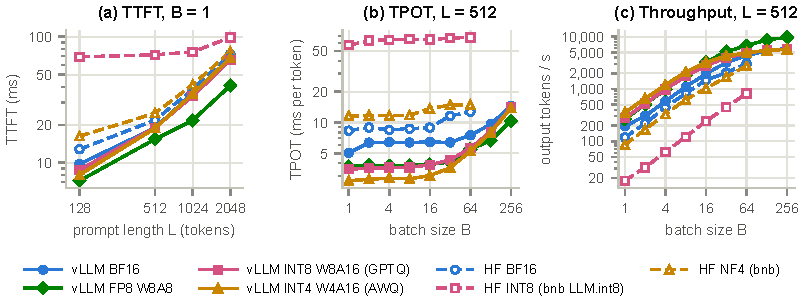
\includegraphics[width=\linewidth]{q2_latency_throughput_3b}
\caption{Latency and throughput of Qwen2.5-3B (same layout as \cref{fig:latency}).}
\label{fig:latency3b}
\end{figure}

\begin{figure}[htbp]
\centering
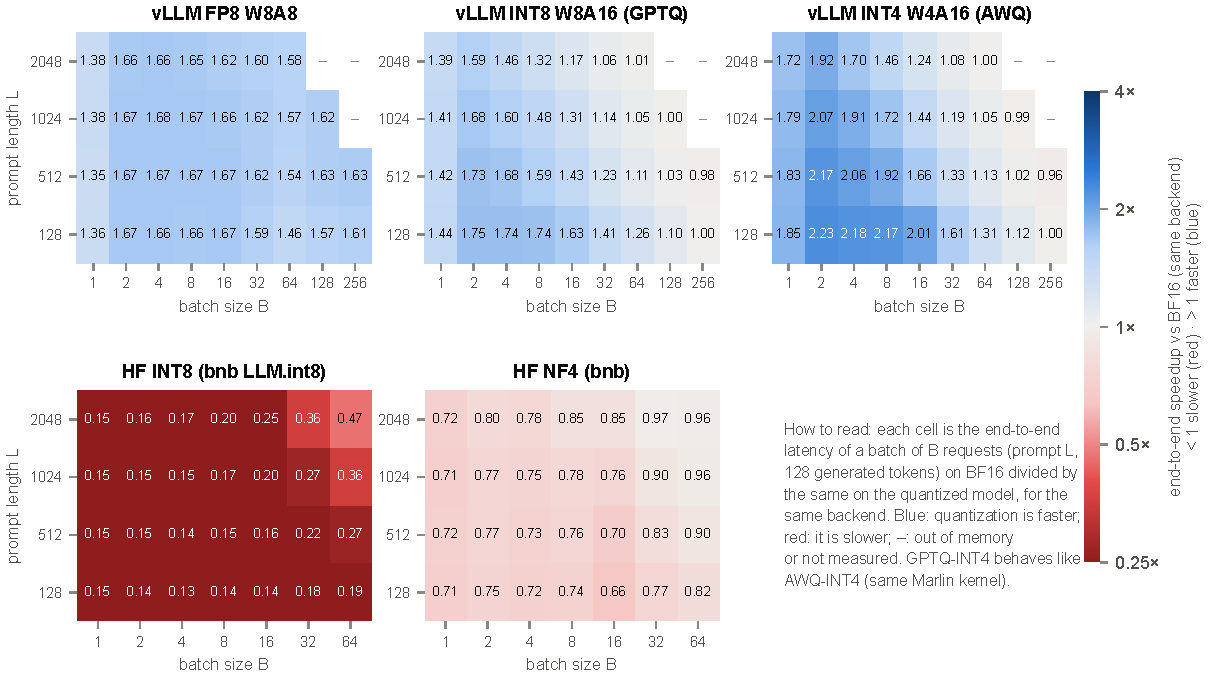
\includegraphics[width=\linewidth]{q3_speedup_heatmaps_3b}
\caption{End-to-end speedup over BF16 for Qwen2.5-3B (same layout as \cref{fig:heatmaps}).}
\label{fig:heatmaps3b}
\end{figure}

\FloatBarrier
\section{Real-traffic details}
\label{app:real}

\Cref{tab:serving_main} summarizes the ShareGPT replay of \cref{sec:real}. \Cref{fig:workload} shows
the lengths of the 300 requests, and \cref{fig:serving,tab:serving} give the full serving results,
including the 99th-percentile latencies.

\begin{table}[htbp]
\centering
\small
\caption{Real traffic: 300 ShareGPT requests replayed against Qwen2.5-7B with their reference answer lengths. $C$ is the number of concurrent requests (HF runs static batches of 16). Output tokens per second, and median TTFT and TPOT in ms.}
\label{tab:serving_main}
\setlength{\tabcolsep}{5pt}
\begin{tabular}{lrrrrrr}
\toprule
 & \multicolumn{2}{c}{$C=1$} & \multicolumn{2}{c}{$C=16$} & \multicolumn{2}{c}{$C=64$} \\
\cmidrule(lr){2-3}\cmidrule(lr){4-5}\cmidrule(lr){6-7}
Config & tok/s & TPOT & tok/s & TTFT & tok/s & TPOT \\
\midrule
HF BF16 (static) & -- & -- & 254 & 797 & -- & -- \\
HF INT8 (static) & -- & -- & 119 & 691 & -- & -- \\
HF NF4 (static) & -- & -- & 215 & 842 & -- & -- \\
\midrule
vLLM BF16 & 104 & 9.6 & 1,334 & 34 & 3,537 & 13.6 \\
vLLM FP8 & 164 & 6.1 & 2,237 & 21 & 5,388 & 8.9 \\
vLLM GPTQ-8 & 166 & 6.0 & 2,166 & 22 & 4,733 & 10.5 \\
vLLM AWQ-4 & 240 & 4.1 & 3,020 & 18 & 5,180 & 10.1 \\
vLLM GPTQ-4 & 241 & 4.1 & 2,970 & 18 & 5,181 & 10.0 \\
\bottomrule
\end{tabular}
\end{table}


\begin{figure}[htbp]
\centering
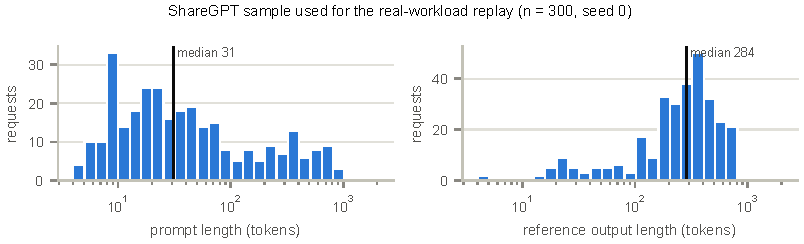
\includegraphics[width=\linewidth]{workload_sharegpt}
\caption{Prompt and answer lengths of the 300 ShareGPT requests used in the replay.}
\label{fig:workload}
\end{figure}

\begin{figure}[htbp]
\centering
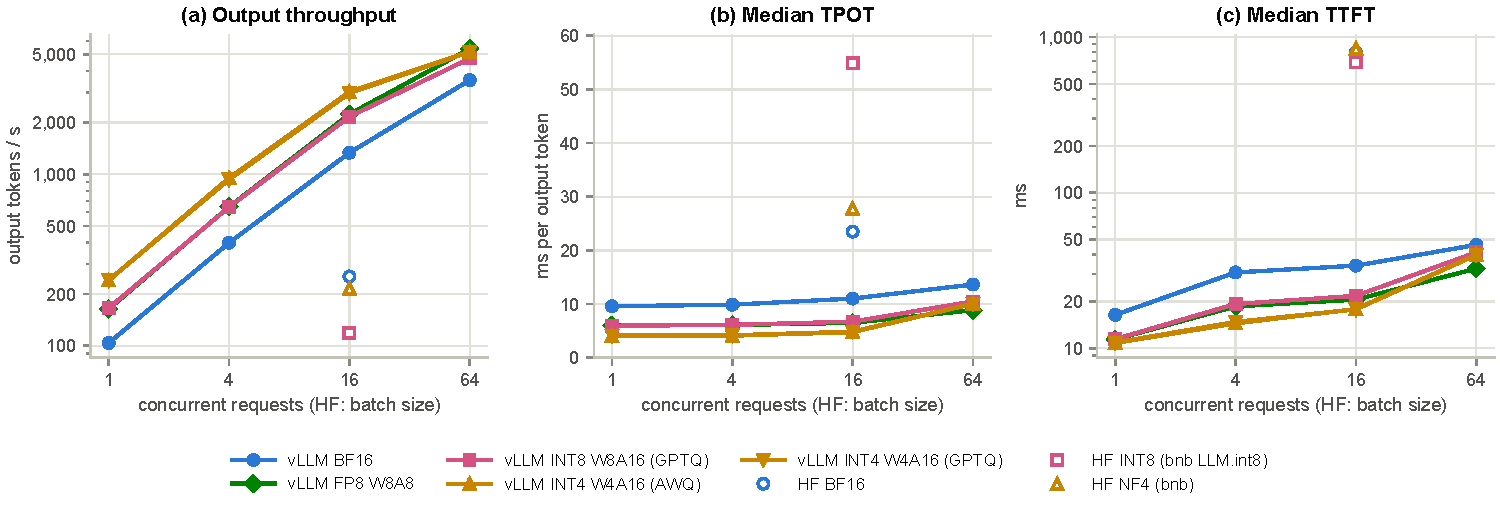
\includegraphics[width=\linewidth]{real_sharegpt_serving}
\caption{The ShareGPT replay against Qwen2.5-7B: vLLM at 1 to 64 concurrent clients (lines) and HF
with static batches of 16 (hollow markers). TTFT and TPOT are medians over requests.}
\label{fig:serving}
\end{figure}

\begin{table}[t]
\centering
\footnotesize
\caption{Real workload --- 300 ShareGPT requests replayed against Qwen2.5-7B (reference output lengths). $C$: concurrent closed-loop clients for vLLM, static batch size for HF. Throughput in requests/s and output tokens/s; TTFT and TPOT in ms.}
\label{tab:serving}
\setlength{\tabcolsep}{3.2pt}
\begin{tabular}{lrrrrr}
\toprule
Config & $C$ & req/s & tok/s & TTFT p50 / p99 & TPOT p50 / p99 \\
\midrule
vLLM BF16 & 1 & 0.35 & 104 & 16 / 62 & 9.6 / 9.6 \\
vLLM BF16 & 64 & 11.76 & 3537 & 46 / 1654 & 13.6 / 16.7 \\
vLLM FP8 & 1 & 0.54 & 164 & 11 / 44 & 6.1 / 6.2 \\
vLLM FP8 & 64 & 17.92 & 5388 & 33 / 1485 & 8.9 / 15.1 \\
vLLM GPTQ-8 & 1 & 0.55 & 166 & 11 / 63 & 6.0 / 6.2 \\
vLLM GPTQ-8 & 64 & 15.74 & 4733 & 41 / 1743 & 10.5 / 18.0 \\
vLLM AWQ-4 & 1 & 0.80 & 240 & 11 / 65 & 4.1 / 4.5 \\
vLLM AWQ-4 & 64 & 17.23 & 5180 & 40 / 1747 & 10.1 / 14.8 \\
vLLM GPTQ-4 & 1 & 0.80 & 241 & 11 / 62 & 4.1 / 4.4 \\
vLLM GPTQ-4 & 64 & 17.23 & 5181 & 40 / 1722 & 10.0 / 19.3 \\
\bottomrule
\end{tabular}
\end{table}


\FloatBarrier
\section{Full quality results}
\label{app:quality}

\Cref{tab:quality} lists every quality number with its $p$-value, for all five models.

\begin{table}[t]
\centering
\footnotesize
\caption{Q4 --- quality. WikiText-2 perplexity (2048-token windows) and GSM8K accuracy (1,319 questions, zero-shot CoT, greedy decoding). Deltas are against HF BF16 of the same model; $p$ is the two-sided exact McNemar test of the paired GSM8K answers against HF BF16.}
\label{tab:quality}
\setlength{\tabcolsep}{3.2pt}
\begin{tabular}{llrrrrr}
\toprule
Model & Config & PPL & $\Delta$PPL & GSM8K (\%) & $\Delta$acc & $p$ \\
\midrule
3B & HF BF16 & 8.56 & -- & 85.8 & -- & -- \\
 & HF INT8 & 8.66 & $+0.10$ & 85.5 & $-0.3$ & 0.777 \\
 & HF NF4 & 9.11 & $+0.55$ & 82.6 & $-3.3$ & $<$0.001 \\
 & vLLM BF16 & 8.56 & $+0.00$ & 86.0 & $+0.2$ & 0.871 \\
 & vLLM FP8 & 8.64 & $+0.09$ & 85.4 & $-0.5$ & 0.610 \\
 & vLLM GPTQ-8 & 8.56 & $+0.00$ & 86.4 & $+0.6$ & 0.322 \\
 & vLLM AWQ-4 & 9.10 & $+0.54$ & 82.7 & $-3.1$ & 0.002 \\
 & vLLM GPTQ-4 & 9.22 & $+0.66$ & 82.0 & $-3.8$ & $<$0.001 \\
7B & HF BF16 & 7.46 & -- & 90.8 & -- & -- \\
 & HF INT8 & 7.49 & $+0.03$ & -- & -- & -- \\
 & HF NF4 & 7.77 & $+0.31$ & 90.3 & $-0.5$ & 0.500 \\
 & vLLM BF16 & 7.46 & $+0.00$ & 91.2 & $+0.4$ & 0.359 \\
 & vLLM FP8 & 7.51 & $+0.05$ & 90.8 & $+0.0$ & 1.000 \\
 & vLLM GPTQ-8 & 7.46 & $+0.00$ & 91.7 & $+0.9$ & 0.043 \\
 & vLLM AWQ-4 & 7.85 & $+0.39$ & 90.4 & $-0.5$ & 0.576 \\
 & vLLM GPTQ-4 & 7.78 & $+0.32$ & 91.1 & $+0.2$ & 0.828 \\
14B & vLLM FP8 & 5.77 & -- & 94.4 & -- & -- \\
 & vLLM GPTQ-8 & 5.71 & -- & 94.7 & -- & -- \\
 & vLLM AWQ-4 & 6.16 & -- & 93.9 & -- & -- \\
 & vLLM GPTQ-4 & 37.46$^{\ddagger}$ & -- & 93.7 & -- & -- \\
\bottomrule
\end{tabular}
\par\vspace{2pt}\parbox{\linewidth}{\scriptsize $^{\ddagger}$Degraded on raw text but not on chat-formatted text; see \cref{sec:q4}.}
\end{table}


\FloatBarrier
\section{Generalization details}
\label{app:general}

\Cref{tab:general} compares Qwen2.5-7B and Qwen3-8B on the same grid.

\begin{table}[htbp]
\centering
\small
\caption{The main results for Qwen2.5-7B and Qwen3-8B (non-thinking mode) on the same grid (512-token prompts, 128 output tokens). Throughput is compared at the largest batch at which both models' KV caches hold every request ($B=64$). Qwen3-8B has no official GPTQ checkpoint.}
\label{tab:general}
\setlength{\tabcolsep}{3.2pt}
\begin{tabular}{lrr}
\toprule
Metric (vs.\ BF16) & Qwen2.5-7B & Qwen3-8B \\
\midrule
Weight saving, AWQ-INT4 (vLLM) & 2.70$\times$ & 2.67$\times$ \\
Weight saving, NF4 (HF) & 2.60$\times$ & 2.55$\times$ \\
Decode speedup $B=1$, AWQ-INT4 & 2.44$\times$ & 2.33$\times$ \\
Decode speedup $B=1$, FP8 & 1.59$\times$ & 1.54$\times$ \\
Decode speedup $B=1$, NF4 & 1.13$\times$ & 0.90$\times$ \\
Decode speedup $B=1$, LLM.int8() & 0.29$\times$ & 0.28$\times$ \\
Throughput $B=64$, AWQ-INT4 & 1.15$\times$ & 1.12$\times$ \\
Throughput $B=64$, FP8 & 1.76$\times$ & 1.67$\times$ \\
GSM8K $\Delta$ pp ($p$), FP8 & $0.0$ (1.000) & $+0.5$ (0.488) \\
GSM8K $\Delta$ pp ($p$), LLM.int8() & $-0.2$ (0.771) & $+0.6$ (0.382) \\
GSM8K $\Delta$ pp ($p$), AWQ-INT4 & $-0.5$ (0.576) & $-0.2$ (0.818) \\
GSM8K $\Delta$ pp ($p$), NF4 & $-0.5$ (0.500) & $+0.2$ (0.909) \\
MMLU $\Delta$ pp ($p$), FP8 & $-0.1$ (0.327) & $-0.7$ ($<$0.001) \\
MMLU $\Delta$ pp ($p$), LLM.int8() & $-0.2$ (0.134) & $+0.7$ ($<$0.001) \\
MMLU $\Delta$ pp ($p$), AWQ-INT4 & $-1.6$ ($<$0.001) & $-0.7$ (0.003) \\
MMLU $\Delta$ pp ($p$), NF4 & $-0.6$ (0.002) & $-0.3$ (0.156) \\
\bottomrule
\end{tabular}
\end{table}


\FloatBarrier
\section{Reproducibility}
\label{app:repro}
Every number in this report is computed from the raw measurements by \texttt{scripts/make\_numbers.py},
and the figures and tables come from \texttt{make\_figures.py} and \texttt{make\_tables.py}.
\texttt{run\_all.sh} runs all experiments again (about twelve GPU-hours on an RTX 5090). A job queue
ran the experiments one at a time, and only while no other user's process was on the GPU. Rows
written while the GPU was shared (\ExcludedWindows, logged in \texttt{results/excluded\_windows.jsonl})
were discarded and those jobs were run again. \RecheckSentence


\end{document}
